%!TEX root = foo-thesis.tex


\chapter{Implementation}
\label{chap:implementation}

This chapter will detail the implementation of the presented techniques. The next two sections will give an overview of the software as a whole and on the rendering pipeline, while the subsequent four sections describe the implementation of the RSM generation, ISM rendering, interleaved sampling, and clustered deferred shading.

The full source code is available in the project's repository\footnote{\url{https://github.com/karyon/multiframesampling}} under the MIT license.


\section{Used Framework and Libraries}

\begin{figure}[htbp]
  \centering
  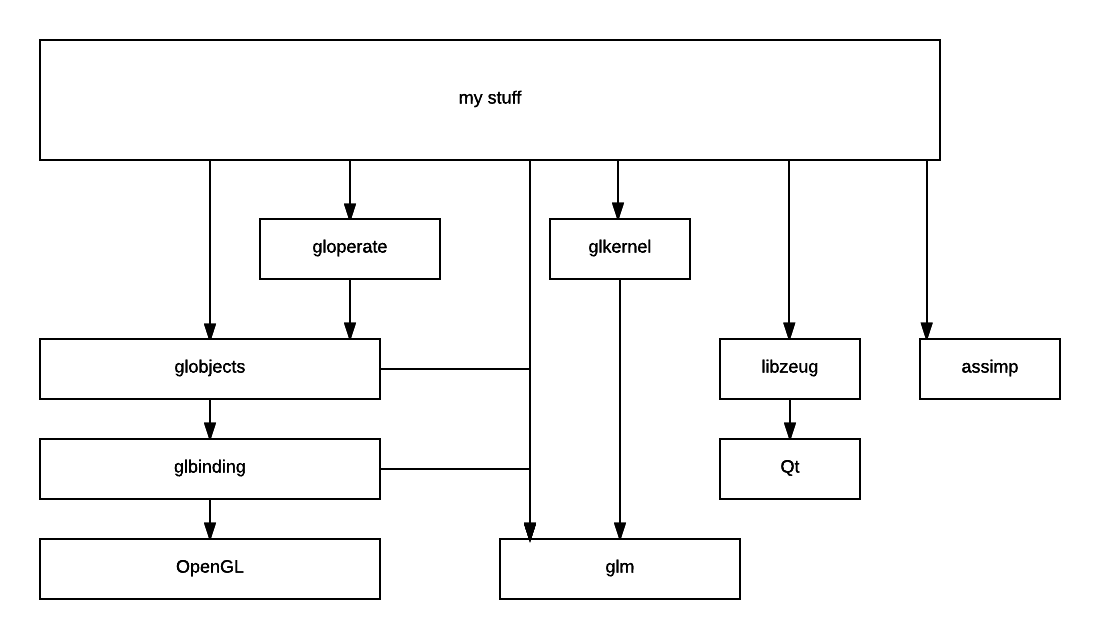
\includegraphics{graphics/Architecture}
  \caption{An overview of the frameworks, libraries and APIs the presented software depends upon.}
\end{figure}

The implementation was built with C++ and OpenGL. It uses \textit{gloperate}\footnote{\url{https://github.com/cginternals/gloperate}} as framework, which provides some basic functionality like navigation and resource handling. \textit{gloperate} in turn is based on \textit{Qt}\footnote{\url{https://www.qt.io/}}, which is used for creating an OpenGL context and the UI. \textit{libzeug}\footnote{\url{https://github.com/cginternals/libzeug}} is used to provide GUI widgets for quick manipulation of the rendering parameters. \textit{globjects}\footnote{\url{https://github.com/cginternals/globjects}} provides a convenience abstraction layer around the OpenGL API, which is in some places directly accessed through \textit{glbinding}\footnote{\url{https://github.com/cginternals/glbinding}}. For math functions and interaction with \textit{globjects}, \textit{glm}\footnote{\url{http://glm.g-truc.net}} is used. Additionally, \textit{assimp}\footnote{\url{http://www.assimp.org/}} is used to load the test scenes.


\section{Rendering Pipeline Overview}

\begin{figure}[h]
    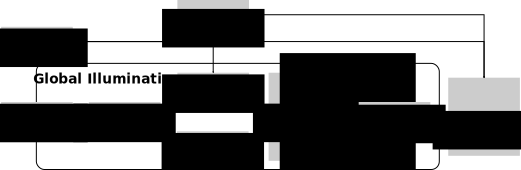
\includegraphics[width=\textwidth]{graphics/rendering_pipeline_overview2}
    \caption{Rendering pipeline overview. The global illumination section is a simplified version of \Cref{fig:GIPipelineConcept}. The RSM rendering does not fully belong to the global illumination section, since it both provides a conventional shadow map for direct lighting, as well as additional information to form a RSM for VPL sampling.}
    \label{fig:RenderingPipelineOverview}
\end{figure}

To provide some context, \Cref{fig:RenderingPipelineOverview} visualizes the complete rendering pipeline of the implemented application. It follows a standard deferred shading approach as it first renders geometry buffers with depth, normal and albedo information and uses these buffers to perform shading in a later stage. In the presented implementation, this stage is simply called ``combine pass'' and computes direct lighting, blends in the results of the SSAO postprocessing, and performs tone mapping that is necessary for HDR rendering. The result of the global illumination is a texture that contains indirect lighting, which is added to the direct lighting in the combine pass.

Most algorithms in this thesis are implemented using OpenGL compute shaders, while the G-Buffer, RSM, and the first stages of the ISM rendering use the regular fixed-function pipeline. The blur pass, SSAO and the combine pass utilize traditional screen-aligned triangles, since compute shaders would provide little benefit for their tasks. Due to the extensive use of compute shaders, OpenGL 4.3 is required to run the application.


\section{RSM Generation and VPL Sampling}
\label{sec:impl:rsmAndVplSampling}

Reflective shadow maps (RSMs) provide a particularly efficient way to create VPLs, since they rely on regular rasterization. As such, the presented implementation of the RSM generation mostly uses the same code as the G-Buffer generation, barring a few modifications: First, normal maps are ignored and triangle normals are utilized instead, and instead of individual texture lookups during shading, the material's average color is used as diffuse color. Both these changes are made in order to avoid high-frequency normal and color changes in the RSM, which can only be captured correctly with a larger number of VPLs.

Additionally, the RSM is re-used as conventional shadow map. Usually, one might want to decouple RSM and conventional shadow map generation to use different resolutions or cascading schemes. It would also be possible to render the RSM with a less detailed version of the scene. Since the presented implementation uses no culling and LOD techniques, it was bottlenecked on geometry complexity. Rendering both RSM and conventional shadow map in one pass is the logical choice in this case. As a result, a variance buffer is rendered in addition to the regular G-buffers for use with the variance shadow mapping technique \citep{Donnelly:2006:VSM}.

Following the RSM generation, a compute shader samples the RSM in a regular pattern and writes the world-space position, normal and color of the sample points into a separate buffer. These information form the VPLs. Additionally, a second buffer is prepared that, instead of one three-component vector for position, normal, and color respectively, stores only one four-component vector in total, holding the VPL's position in the first three components and the normal packed into the last component (\citet{Cigolle:2014:NormalPacking}). This is done because the ISM rendering (\Cref{sec:impl:ismRendering}) and light list calculation (\Cref{sec:impl:clusteredShading}) do not need the color information and especially the ISM rendering reads several VPLs per point, using a lot of bandwidth.


\section{ISM Rendering}
\label{sec:impl:ismRendering}

For rendering imperfect shadow maps, a set of points is first generated from the scene geometry. This process is detailed in the next subsection. Subsequently, for each imperfect shadow map a random subset of points is chosen and rendered using a paraboloid projection. To this end, two different approaches, the splat and single-pixel renderer, have been presented in the previous chapter. Their implementation is described in \Cref{sec:impl:splatting,sec:impl:singlePixelRendering}. Subsequently, the pull-push postprocessing required by the single-pixel renderer is detailed.

\subsection{Point Generation}
\label{sec:impl:pointGeneration}

We make use of OpenGL's tessellation shader to subdivide triangles to make them meet a certain maximum size. The tessellation control shader determines the tessellation levels according to the triangle's size. The tessellation evaluation shader does nothing more than correctly interpolating the vertex positions. The geometry shader, which now receives the smaller, tessellated triangles, converts each triangle to a point. The point's center equals the triangle's center, and the radius is chosen to make the areas of the point and triangle match. Note that no translation or projection has been applied yet, this is done in a later stage.

While a random subset of all points needs to be chosen for each ISM, special attention must be paid to ensure that each individual ISM uses the same subset of points across different frames. Otherwise, the ISMs will be temporally incoherent and cause flickering in the final rendering. To this end, each point's barycentric coordinate inside its triangle and the triangle's \texttt{gl\_PrimitiveID}\footnote{\url{https://www.opengl.org/sdk/docs/man4/html/gl_PrimitiveID.xhtml}} are passed to a fast hashing algorithm. The result is used to determine an ISM ID (or, equivalently, a VPL ID) per point. How the ISM ID is used depends on whether point splatting or the single-pixel renderer is enabled.



\subsection{Point Rendering with Splatting}
\label{sec:impl:splatting}

In the case of point splatting, the geometry shader itself reads the VPL with the ID it determined, projects the point according to the VPL's data, performs culling, and discards the point if necessary, sets \texttt{gl\_PointSize} to the correct size after projection, and emits a vertex. To prevent the GPU from assembling triangles from the geometry shader output and render point splats instead, the \texttt{output\_primitive} must be set to \texttt{points} in the geometry shader's \texttt{layout}\footnote{\url{https://www.opengl.org/wiki/Geometry_Shader\#Primitive_in.2Fout_specification}} definition. As explained previously, for point splatting all points are simply enlarged by a small constant factor in lieu of the pull-push postprocessing. Since only depth information are needed in this case, the fragment shader is empty.



\subsection{Single-Pixel Point Rendering with Compute Shaders}
\label{sec:impl:singlePixelRendering}

This alternative approach was inspired by the fact that the surface reconstruction algorithm proposed by \citet{Marroquim:2007:reconstruction} works with single-pixel ``splats''. Since in this case the hardware rasterizer is not required to achieve good performance, this allowed for more flexibility and new optimization opportunities.

\subsubsection{Approach}

The general idea is to first let the geometry shader write the generated points into a buffer, which is then used by a separate compute shader pass to perform the actual rendering. However, in order to maintain temporal coherence, the points are not written into a single large buffer, as it would be hard to determine a location consistent across frames for each point in that buffer. Instead, the buffer is divided into one partition per VPL, and the points are written into the partition corresponding to the ID calculated before. An atomic counter that indicates the first free index is used per partition to sequentially fill these partitions without overwriting any data. The order of the points within each partition is undefined, but that does not change the output since they all are going to be rendered into the same ISM.

After the point buffer has been prepared, a compute shader is used to render the points. For each VPL, one work group reads through the respective partition of the point buffer and performs the transformation and culling against the VPL for each point. It then calls \texttt{imageAtomicMin}\footnote{\url{https://www.opengl.org/sdk/docs/man/html/imageAtomicMin.xhtml}} to ``render'' the point with correct depth testing as a single pixel into the respective ISM. Since atomic operations operate on single channel integer textures only, it is not possible to use a second or third channel for additional attributes. Instead, one 32 bit channel is used, with 24 bits containing the depth, and 8 bits containing the radius. Since the depth is contained in the 24 more significant bits, the depth test still works correctly. Another version that used a 3D texture for additionally storing the normal was implemented as well, see the next subsection.

As an optimization, the compute shader renders each point into several ISMs. To this end, each work group reads the data of a fixed number of VPLs (e.\,g., 16) into shared memory. Then, while rendering the points, culling is performed per point on all 16 VPLs, and those VPLs where the point passes the culling test are collected into a local array. Thereafter, the point is transformed for each of the collected VPLs and rendered into the respective ISM. While this approach made the compute shader renderer more efficient, an attempt to implement the optimization for the splat renderer by emitting multiple vertices in the geometry shader resulted in a significant performance hit (\Cref{sec:results:ism:performance}).


\subsubsection{Challenges when using a second render target}
\label{sec:impl:raceCondition}

For a higher-quality postprocessing, the normals of the points are required. Since we did not use the normals in our final version, we were able to follow the simplified one-channel approach described above, but we had implemented a different version that also stored normals. To this end, the ISM texture was made three-dimensional, and the second index of the third dimension was used as additional ``render target'' to hold the radius and normal. The issues we faced during the development are described here.

In addition to roughly doubling the time needed to render the points due to the increased bandwidth, this approach introduces a second race condition besides the usual z-fighting that can occur. If two threads with differing depth values simultaneously write into the depth buffer, using \texttt{imageAtomicMin} guarantees the correct value will end up in the buffer. However, if the higher value is written first and subsequently is overwritten by the second write, both writes have in fact succeeded. This results in both threads attempting to write into the second buffer, creating a race condition since the execution order of the writes is undefined. This problem can be alleviated by adding a synchronization point after the atomic write and by then reading the memory location that has just been written to. If it is equal to the written value, one can assume the write actually succeeded and was not overwritten by a second, simultaneous write. Only then the write to the second buffer is performed.

This solution had little cost (12\,\% of the point rendering or 3\,\% of the total ISM rendering time), but it fixes the race condition only inside one work group and not between work groups, for which there are no efficient synchronization primitives on the GPU. On a NVIDIA GTX 750 Ti, the race condition was still observable but acceptable. Interestingly, on a GTX 980, the race condition seemed not to occur at all with the described workaround.

\citet{Günther:2013:AcceleratedPointCloudRendering} propose to double the texture size of the depth buffer and use each second texel as lock with the help of OpenCL's \texttt{atomic\_cmpxchg}\footnote{\url{https://www.khronos.org/registry/cl/sdk/1.2/docs/man/xhtml/atomic_cmpxchg.html}} function (\texttt{atomicCompSwap}\footnote{\url{https://www.opengl.org/sdk/docs/man/html/atomicCompSwap.xhtml}} in GLSL) to write both depth and additional attributes without race conditions. A more elaborate solution that might open  even more optimization opportunities would involve a more advanced software renderer, e.\,g., following the approaches of \citet{Laine:2011:SoftwareRasterization}.


\subsection{Pull-Push Postprocessing}
\label{sec:impl:pullPushPostprocessing}

Our implementation of the pull-push algorithm to reconstruct surfaces from single-pixel points is relatively straightforward. For each miplevel to be calculated, one \texttt{dispatchCompute}\footnote{\url{https://www.opengl.org/sdk/docs/man4/html/glDispatchCompute.xhtml}} is called. Since the first step of the pull phase has different inputs than the subsequent steps (its only inputs are depth and size, not the displacement vector and depth interval), a slightly different shader is used there. Analogously, the last step of the push phase outputs only depth, therefore a shader variant is created for that step as well. For the same reason, the initial input texture (the ``render target'' used by the single-pixel renderer) and final output texture (the finished ISM used later for shadowing) have different formats than the mipmap levels used by the pull-push algorithm.


In the pull phase, one compute shader invocation calculates one output pixel. It reads its four input pixels, determines which of them are valid, and uses the valid ones with equal weights for interpolating.


During the push phase, groups of four output pixels share the same input pixels. This can be exploited by letting each shader invocation compute four output pixels while still reading only four input pixels. Naturally, the weights applied to the input pixels need to be adjusted per output pixel. For invalidating input pixels, their weights can simply be set to zero instead of separately marking them as invalid.

Note that there is still lots of room for optimization. Especially the pull phase is basically a parallel reduction which is well-researched and for which optimized algorithms on the GPU are available (\cite{Harris:2007:ParallelReduction}). Several optimizations from that field might be applicable here.



\section{Interleaved Sampling using Compute Shaders}
\label{sec:impl:interleavedShading}

The presented implementation performs interleaved sampling, that is, it processes only a fraction of all VPLs per pixel and uses a blur pass to mask the resulting noise. Since adjacent pixels now process different sets of VPLs, this approach results in low cache coherence. To this end, de-interleaving is employed \citep{segovia2006non}.

Often, de-interleaving is implemented by splitting the G-buffer into several smaller buffers, each containing all pixels with the same sample set. Each buffer is processed with its respective sample set, and then the buffers are re-interleaved into a large G-Buffer again.

We propose to perform de-interleaving, sample processing, and re-interleaving in a single pass using compute shaders. Just like the original method, this approach allows for cache-efficient processing since each work group processes a set of pixels that have the same set of VPLs assigned. However, instead of splitting the G-Buffer and then re-interleaving it to perform coherent reads and writes, we propose to let the compute shader read and write directly to the respective pixels in the G-Buffer.

There are several reasons for this approach: First, implementation complexity is reduced, since the buffer splitting and re-interleaving phases are not needed as separate shader passes anymore. Second, as another consequence of eliminating these phases, the total amount of memory read and written is greatly reduced, potentially saving bandwidth. And third, no additional storage is needed.

A potential downside is that this technique performs one scattered read of the G-Buffers, compared to several coherent reads performed by the buffer splitting method. However, the bottleneck of the final gathering phase lies within the loop over the VPLs, therefore an initial one-time scattered read is likely to not have any impact but to be swallowed by latency-covering techniques of the GPU. Theoretically, the work groups could be distributed over the GPU's processor clusters (Streaming Multiprocessors on NVIDIA, Compute Units on AMD) in a way that adjacent pixels are still processed on the same cluster, but unfortunately, application developers have no control over this.

Since only a subset of all samples is processed per pixel and this subset repeats every few pixels, interleaved sampling results in structured noise. To this end, a bilateral blur similar to \citet{laine2007incremental} is often used. The blur filter is bilateral, i.\,e. it takes depth and normal discontinuities into account, to prevent light from bleeding over geometry edges. Although bilateral filters are in fact not separable, they are commonly implemented in a separated fashion. This trades a negligible quality impact for large performance benefits, and the presented implementation follows this approach.


While the bilateral blur achieves close to perfect results on even surfaces, the structured noise is harder to mask along geometry edges due to missing information. This problem becomes even more apparent when using regular VPL sampling, which makes each pixel process VPLs that are near each other. For example, this might result in the first pixel inside a 4x4 block processing VPLs that are near the pixel's location, while the second pixel processes VPLs that are all farther away, causing the differences between the pixels to be amplified. To this end, the order of the VPLs in the VPL buffer created during the VPL sampling phase is simply shuffled, using a fixed permutation precomputed on the CPU. See \Cref{sec:results:interleavedShading} for the effects of this small optimization.

Instead of shuffling, an interesting and more elaborate solution to make the noise easier to mask are Metalights \citep{Faure:2010:Metalights}. They sort the VPLs after their contribution to the image and pick a representative subset per pixel. While the blur is still necessary, this might provide better results for problem cases such as thin structures.


\section{Clustered and Tiled Deferred Shading}
\label{sec:impl:clusteredShading}

Since both tiled and clustered deferred shading discard lights only if they do not contribute any light energy to a cluster of pixels, they never alter the rendered output when implemented correctly and purely affect performance. Nevertheless, there are several implementation choices to be made.


\subsection{Clustered Deferred Shading}

The presented implementation of clustered deferred shading uses 128 pixels as screen-space tile size and 16 depth slices. It also draws on an optimization proposed by \citet{persson::2013::practical} by using a larger near cluster for better depth slice utilization.

In some situations it is advantageous to perform the light assignment step on the CPU as done by \citet{persson::2013::practical}. In their context of computer games, they have mostly small light radii, making it possible to quickly determine the clusters that are reached by a certain light. For global illumination, however, infinite light radii are preferred, resulting in a higher number of clusters that are reached by each light source. Therefore, starting with all clusters that contain fragments and iterating over all lights for each cluster becomes viable, as opposed to determining the set of reached clusters per light. The more uniform control flow of this approach makes it a reasonable choice to use GPUs for the light assignment step. Additionally, since the lights are already generated on the GPU during the RSM sampling phase, CPU-side culling would require copying light data to the CPU and culling results back; performing culling on the GPU eliminates these data transfers.


The clustered shading technique is divided into three phases: clustering, light assignment and shading. Each of these corresponds to one compute shader dispatch call.

\paragraph{Clustering.}
In this step, each work group processes one 128²\,px screen-space tile. Since the number of threads in a work group is limited, each thread in the work group iterates over several fragments. For each fragment, the corresponding depth slice is determined and marked as used in a shared array of 16 booleans. Since no thread writes False or reads from the shared array, no data races can occur and no synchronization is needed in this step.

Now the work group counts the number of used depth slices. This can be done with 16 threads, utilizing atomic increment operations on a shared variable, or one thread that iterates over the sixteen booleans. Since both ways take a negligible amount of time, the choice does not matter in practice.

The number of used depth slices is then added to one global atomic counter. The corresponding GLSL function (\texttt{atomicAdd}\footnote{\url{https://www.opengl.org/sdk/docs/man/html/atomicAdd.xhtml}}) returns the value of the counter before the addition. This way, each work group ``allocates'' some space in a global list of used clusters. It then writes an ID identifying each cluster into the allocated section in that list. To be able to later determine a cluster's position in the global list, a 3D texture with one texel per cluster is filled with each cluster's location.

Instead of a compact list of used clusters and a compact texture of light lists, one could omit the list of used clusters and employ a sparse texture of light lists where the light list of each cluster has a fixed position. However, this would obviously require more memory, even if only a few megabytes, since most parts of the light list texture would be unused. It would also make the light assignment step more inefficient, since it would become necessary to test for each cluster whether it is used, instead of simply processing a compact list of used clusters.


\paragraph{Light assignment.}
With a new dispatch call, each thread now performs culling for one light and one cluster. Given the cluster coordinates, it reconstructs the cluster's bounds and checks on which side of the plane described by the VPL's position and normal the cluster is located. More specifically, if any of the cluster's eight corners is on the illuminated side of the VPL, the light cannot be culled and is added to the light list of the cluster.

The light lists are stored in a 2D texture with a height of the maximum amount of clusters and a width of the number of VPLs. The $n$th row in that texture contains the light list of the cluster at index $n$ in the global list of used clusters created in the previous step. Additionally, each light list is divided into 16 partitions, one partition for each pixel in an interleaving block. See \Cref{fig:impl:light_lists} for a visualization of this texture. The partitioning not only simplifies the light list lookup during shading, it also guarantees that each light is processed exactly once in an interleaving block.

\begin{figure}[h]
    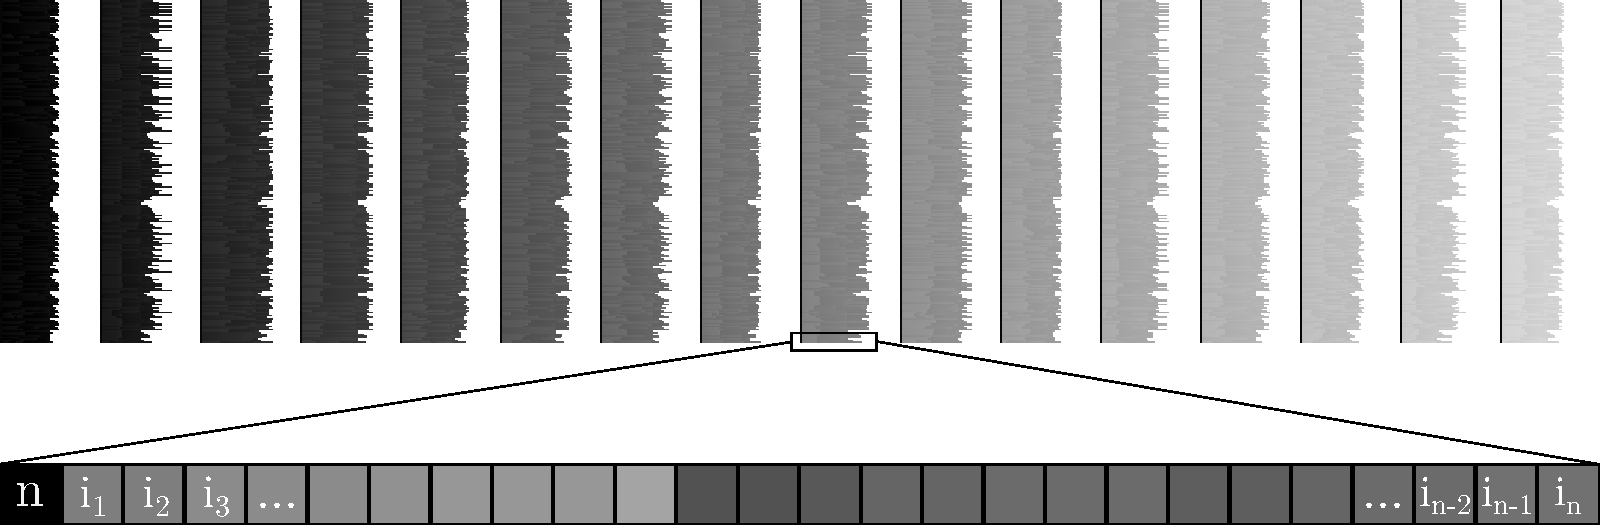
\includegraphics[width=\textwidth]{graphics/light_lists}
    \caption{Visualization of the light lists texture. Each pixel row contains the light list of one cluster. The lists are divided into 16 partitions, one for each pixel in an interleaving block. Each red pixel represents an index to an VPL, a brighter red is a higher index. White pixels contain no data. The first value in each partition is the number of lights in that partition, therefore the dark line in front of the partitions.}
    \label{fig:impl:light_lists}
\end{figure}

As a simplified example, suppose that only four lights are used and the interleaving block size is 2x1, i.\,e., that it contains only two pixels. As described in the interleaved sampling algorithm, in this case the first pixel will process the first half of its light list, while the second pixel will process the second half of its respective light list. If the first pixel's light list contains lights 3 and 4, while the other pixel is in a different cluster whose light list contains lights 2 and 3, then for both pixels only light 3 will be processed. As a result, one light will have been accounted for twice, while two other lights have not been considered at all. This was visible as darkened or brightened lines along the screen-space tiles used by the clustered shading algorithm. The partitioning scheme completely fixes this by guaranteeing that the first pixel always processes lights 1 and 2, while the second pixel always processes lights 3 and 4, minus culling results respectively.

While the partitions cannot reasonably be shrinked much, one could estimate the average of used depth slices per tile to reduce memory consumption. Since the list of used clusters is stored in a compacted list as discussed previously, individual tiles can still use more depth slices than estimated and not break the algorithm. An average of 4 out of 16 depth slices is likely enough for most scenes and would cut down the memory consumption of the light list texture by 75\,\%. To provide a reference: Since each partition contains only 64 lights, 8-bit indices are sufficient. The light list of each cluster thus needs 1\,KB. For a full HD resolution and screen-space tiles of 128\,px, the maximum number of clusters is 2160, thus a little over 2\,MB of memory is needed. With the discussed estimate of 4 used clusters per tile, this can be cut down to 540\,KB.

\paragraph{Shading.}
The final gathering shader processes one pixel per invocation. Without clustered shading, each invocation simply processes the subset of VPL's that should be used as determined by the interleaved sampling algorithm. With clustered shading, it will instead first determine the pixel's cluster and subsequently process the lights in this cluster's light list and in the partition corresponding to the pixel's position in its interleaving block.


\subsection{Tiled Deferred Shading}

In addition to clustered deferred shading, we also implemented its predecessor tiled shading. Since tiled shading does not perform clustering in the z-dimension (or in other words, it uses only one depth slice per tile), it allows for a simpler implementation.

We integrated tiled shading directly into the final gathering shader, in an approach very similar to \citet{Andersson:2011:RenderingBattlefield3}. As a reminder, during final gathering each work group processes those pixels from several interleaving blocks that process the same set of VPLs, and each invocation processes one pixel. With tiled shading, each pixel's z-value is used to build a minimum and maximum z-value for this work group, utilizing atomic operations. In a second step, each invocation processes one VPL and culls it against the bounding box of the pixels, which is defined by the pixel's minimum and maximum fragment coordinates and z-values determined in the previous step. All lights that pass the culling test are added to a light list in a shared array, again utilizing atomic counters to ensure no gaps are produced and no light is overwritten. Subsequently, final gathering is performed as usual with the difference of reading from the light list in the shared array instead of a light list computed in a previous shader pass.

Similar to the integrated interleaved sampling algorithm, this implementation has several benefits. Again the implementation complexity is reduced, since no additional shader passes and no additional buffers with corresponding data layout considerations are needed. Second, no additional storage is needed, and third, this implementation, although simpler, turned out to be faster than clustered deferred shading. See \Cref{sec:results:clusteredShading} for details.
